% Figure block for the DATA-SCALING analysis (fig_mm_consumption.pdf) — the consumption axis.
% Distinct from fig_mm_scaling, which is now only the fixed-compute CONTROL (pool size).
%
% REPRO(fig:mm_consumption):
%   MMRAG_DATA=<data> python3 mmrag/plot_scaling.py --consumption-out mmrag/fig_mm_consumption
% x = unique examples consumed = batch_size (4) x steps; checkpoint evals named <parent>-ck<STEP>
% inherit the parent's config and contribute STEP x batch_size. Series are pinned to the pool
% sizes in CONSUMPTION_AVAIL so every point is no-reuse and from one query distribution
% (v1: the 200k pool only; v3 additionally the 45,248 headline cell -- flagged in the prose as a
% different distribution from its own continuations). max_steps is FREE on this axis (it IS the
% axis) and pinned on the pool-size axis; the two collectors deliberately differ.
% The script refuses to emit until a series has >=3 points, so a 2-point "curve" cannot ship.
% Dashed overlay = best-so-far envelope, so a run past its peak cannot read as data-limited.
%
% Values at the commit that produced the current PDF (v1 fresh, 200k pool):
%   2k scale-rows200k 0.3480 | 6k scale-rows200k-s1500(+ -s1) 0.3457 (2 seeds) |
%   12k scale-rows200k-s3000 0.3307;  v3 fresh: 2k v3-pure x3 0.3471
% IN FLIGHT: v1 scale200k-ck{250,500,1000,1500,2000,2500} (the dense curve),
%   v3 v3-rows200k-s1500 (6k, job 749f47f6) and v3-rows200k-s3000 (12k, job e89a2ad8).
% Regenerate when they land -- the figure picks them up with no edit to the script.
\begin{figure}[t]
\centering
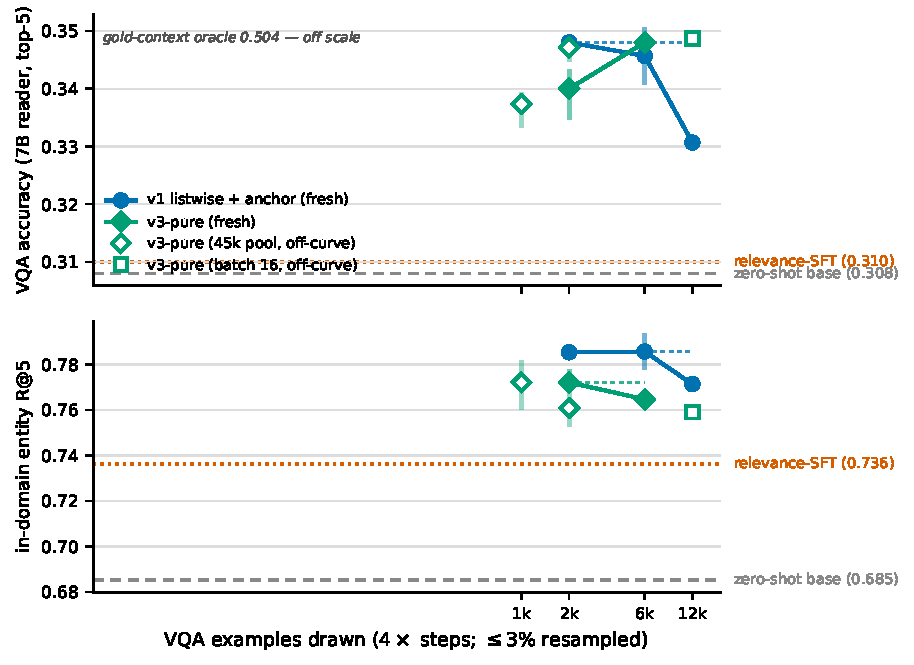
\includegraphics[width=0.66\textwidth]{fig_mm_consumption.pdf}
\caption{\textbf{Data scaling on the axis that matters: examples actually consumed.} Downstream
VQA accuracy against the number of unique (image, question, answer) triples the run has consumed
(batch $\times$ steps), holding the model (\textsc{GME-Qwen2-VL-2B}) and the recipe fixed and
drawing from the $200$K pool so that no example is reused. Compute follows data by construction,
so this is the curve that answers ``does collecting more cheap VQA supervision buy accuracy?''
--- unlike the fixed-compute control in Figure~\ref{fig:mm_scaling}, where enlarging the pool
changes nothing because the consumed count does not move. Dashed overlay is the best-so-far
envelope, drawn so that a run past its peak cannot be misread as data-limited. \textbf{The dense
intermediate-checkpoint cells are still in flight}; the points shown are final-step runs, and the
paragraph text states in advance how either shape will be read.}
\label{fig:mm_consumption}
\end{figure}
